\chapter{Tire Model Exercises - 1}

\section{Exercise 1 – Pure Longitudinal Slip}
\textbf{Q. Using the Pacejka Magic Formula, plot the longitudinal tire force $\fxz$\ obtained in pure longitudinal slip conditions, as a function of slip $\kappa$ $\in$ [−1, 1]. Which comments are you able to make about the obtained graph?}
        \begin{figure}[h]
        \includegraphics[scale=0.5]{ex1/e-11.eps}
        \centering
        \caption{$\fxz$ as a function of slip}
        \end{figure}

When $\kappa$ (longitudinal slip) increases, $\fx$\ grows until it reaches a saturation limit. Furthermore, the slip zone grows, and the adherence area decreases. That means, the total tire force $\fx$\ keeps growing until it reaches a peak and a saturation limit as shown in the graph below. $\kappa$ (longitudinal slip) is positive when the tire is accelerating, negative during braking, and reaches -1 when the wheel locks.
        \begin{figure}[ht]
        \includegraphics[scale=1]{ex1/e-12.png}
        \centering
        \caption{Slip and adherence forces}
        \end{figure}


\textbf{Q. If you were supposed to design a traction control system for maximizing vehicle longitudinal acceleration, which would be the target value of longitudinal slip $\kappa$ that you would try to achieve?}

Acceleration is directly proportional to the force [F=ma] if the mass is constant. If I want to maximize the vehicle longitudinal acceleration, I would need to maximize the longitudinal force [$\fx$]. $\fx$\ is highest at the saturation limit, which in this example happens at slip $\kappa$ = 0.094, and yields an $\fx$\ of 2022.99 N.

\textbf{Q. Assuming that wheel rotational speed is $\omega$ = 70 rad/s, tire effective rolling radius is R$_{e}$ = 0.2 m, while the longitudinal component of tire contact point speed $\vcx$\ = 13 m/s, compute the longitudinal slip $\kappa$. In these conditions, is the wheel accelerating, braking or is it in pure rolling? Compute also the corresponding longitudinal tire force $\fxz$}

Using Matlab, the calculated longitudinal slip $\kappa$ = 0.0769 and the calculated longitudinal force $\fx$\ is = 1990.65 N. the longitudinal slip is positive ($>$0), which means that the wheel is accelerating.

\textbf{Q. Compute the cornering stiffness Cf$\kappa$, that is the derivative for $\kappa$ = 0 of the $\fxz$. Up to which value of $\kappa$ is the linear approximation of Pacejka curve acceptable?}

The cornering Stiffness Cf$\kappa$ is equal to the derivative of the longitudinal force with respect to the longitudinal slip when the longitudinal slip is equal to zero. This means its equal to the slope at the origin (x=y=0) or equal to BCD function as shown in Figure \ref{co-st}. The calculated cornering stiffness is Cf$\kappa$ = 47909.4

        \begin{figure}[ht]
        \includegraphics[scale=1.2]{ex1/e-13.png}
        \centering
        \caption{cornering stiffness as a linear approximation}
        \label{co-st}
        \end{figure}
        
The linear approximation allows to neglect the complex Pacejka Magic Formula, but it is valid only for small $\kappa$. At $\kappa$ = 0.02, the percent difference is already at 10\% as shown in Figure \ref{pd-p}.

        \begin{figure}[ht]
        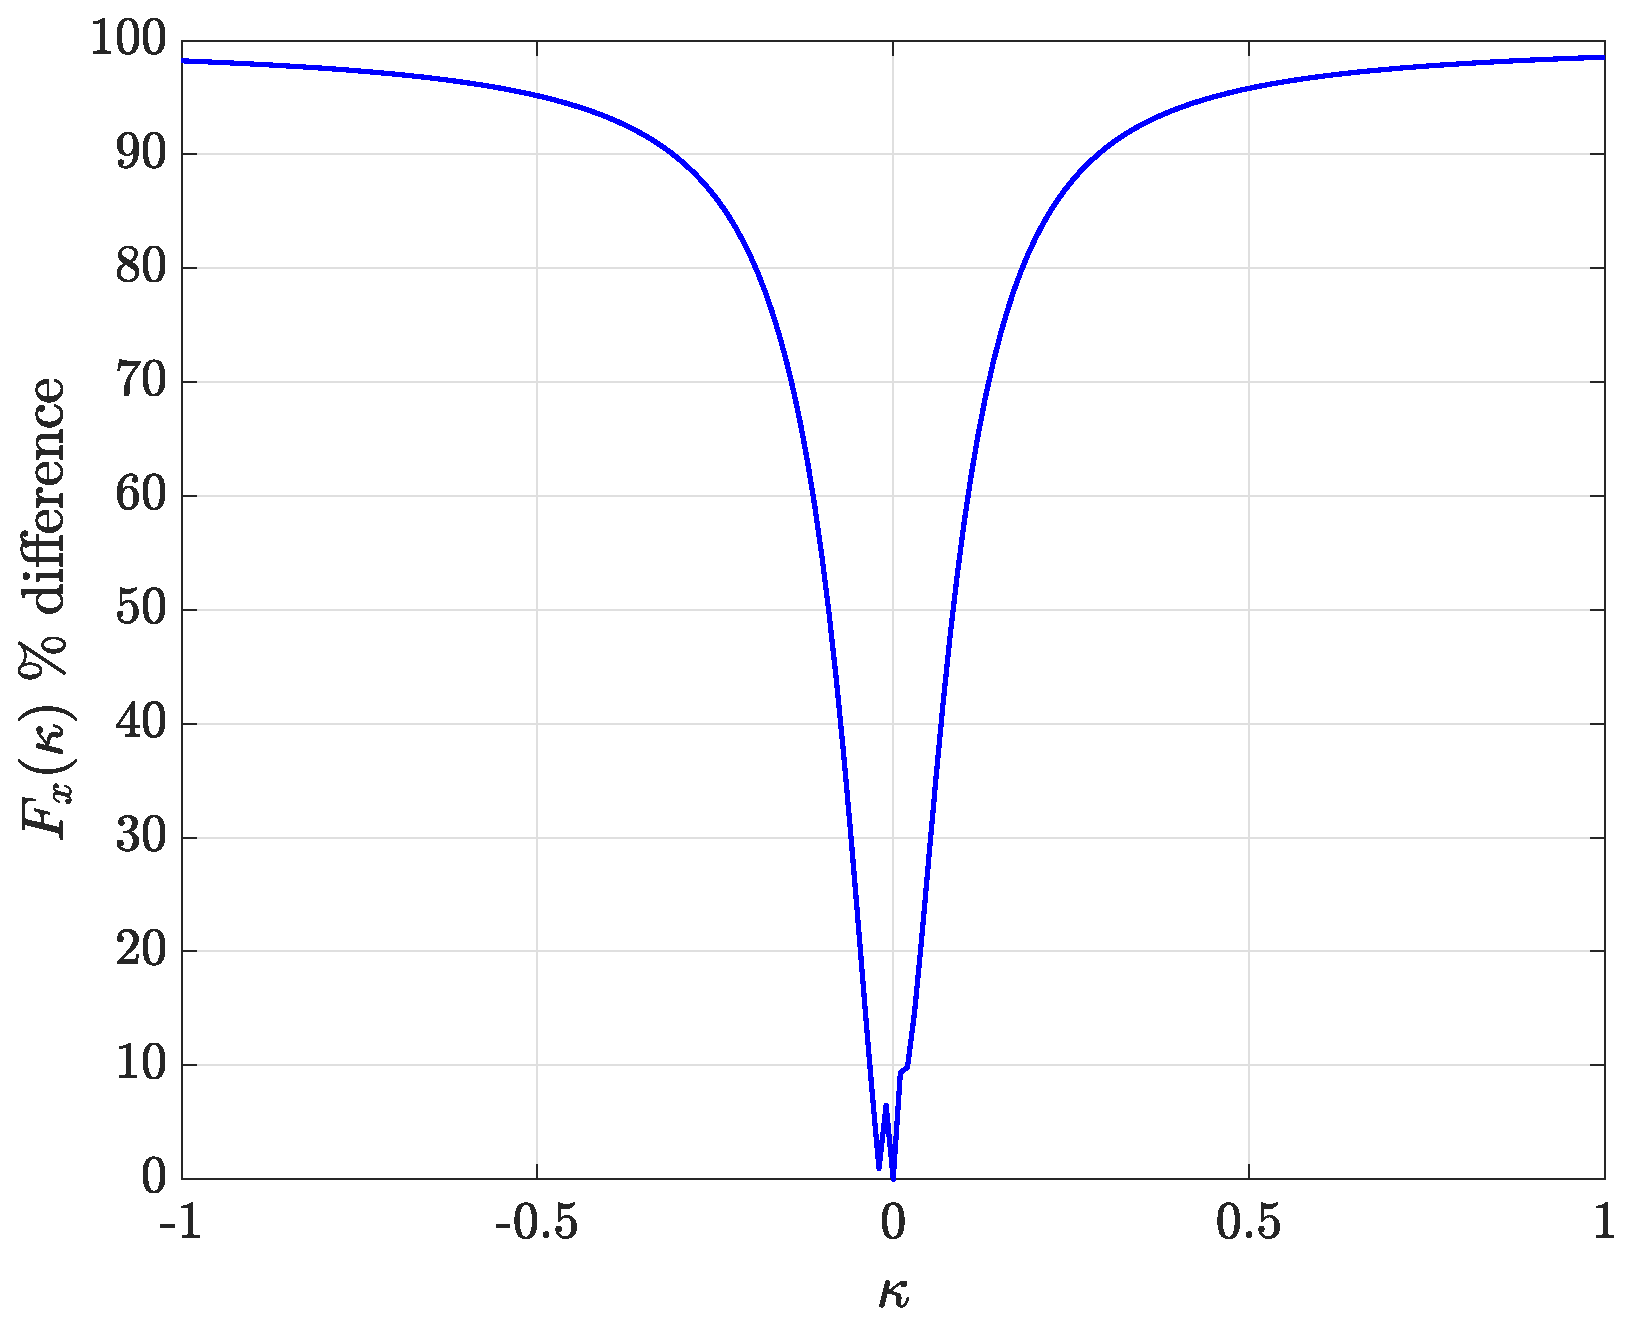
\includegraphics[scale=0.5]{ex1/e-15.eps}
        \centering
        \caption{\% difference in $\kappa$ using linear approximation vs Pacejka formula}
        \label{pd-p}
        \end{figure}

\newpage

\section{Exercise 2 - Combined Slip}

\textbf{Q. Assume that the tire contact point velocity components along the tire x and y axes are $\vcx$\ = 15 m/s and $\vcy$\ = −1.3 m/s, respectively. Calculate the side slip angle $\alpha$. Moreover, compute the combined tire force $\fx$\ using this value of $\alpha$, for a longitudinal slip $\kappa$ = 0.08.}

Alpha can be calculated using the practical slip approach:

\begin{equation}\label{eq:1.1} % add * after equation for unnumbered equations
    \mbox{side slip angle  }  \alpha = - \arctan(\frac{\vsy}{\vcx}) = - \arctan(\frac{\vcy}{\vcx})
\end{equation}

Using equation \ref{eq:1.2} to calculate $\gxa$\ (weighing function). Once calculated, $\fxz$\ can now be multiplied by $\gxa$\ (weighing function) to get the combined tire force $\fx$.

\begin{equation}\label{eq:1.2} % add * after equation for unnumbered equations
    \gxa = - \dxa \cos(\cxa \arctan(\bxa(\alpha + \shxa))
\end{equation}{\vspace{-4em}}

\begin{equation}\label{eq:1.3} % add * after equation for unnumbered equations
    \fxz = \dx \sin(\cx \arctan(\bx \kx - \ex(\bx \kx - \arctan(\bx \kx)))
\end{equation}{\vspace{-4em}}

\begin{equation}\label{eq:1.4} % add * after equation for unnumbered equations
    \fx = \gxa \fxz
\end{equation}

Using Matlab to calculate the side slip angle $\alpha$ and combined tire force:

{\centering\fbox{\begin{minipage}{20em}
calculated side slip alpha = 0.086451 \\
calculated weighing function = 0.724417 \\
calculated combined force $\fx$\ = 1450.424623
\end{minipage}}\par}

\textbf{Q. Plot the combined longitudinal tire force $\fx$\ as a function of $\kappa$ $\in$ [−1, 1], for the following levels of side slip angle $\alpha$ = \{0, 2, 4, 6, 8\} degrees. Which comments can you make about the 5 curves obtained in this way? Finally, plot the weighting function $\gxa$\ as a function of $\kappa$ $\in$ [−1, 1] for each of the previously defined values of $\alpha$, and briefly comment also these 5 curves.}

Figure \ref{clf} shows plots obtained for the combined longitudinal force $\fx$\ for each side slip angle as a function of the longitudinal slip $\kappa$. The maximum combined longitudinal force $\fx$\ keeps decreasing with higher side slip $\alpha$.\newpage

        \begin{figure}[ht]
        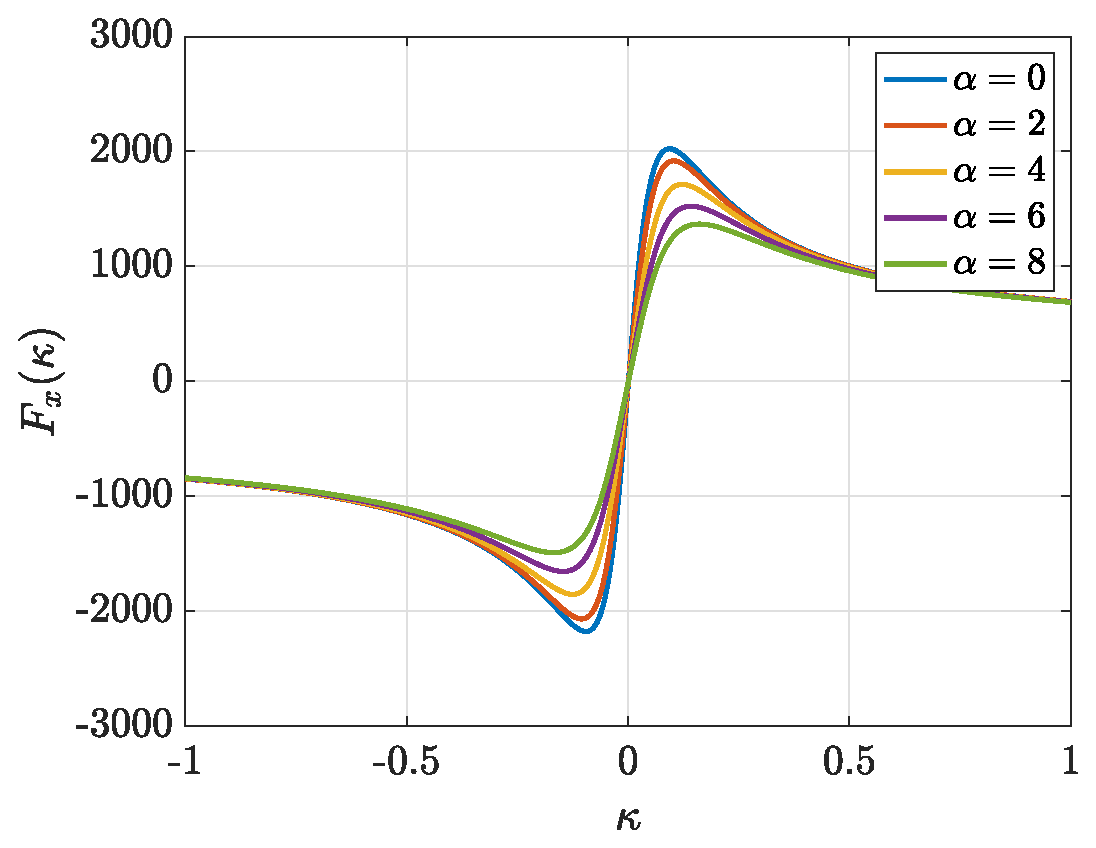
\includegraphics[scale=0.5]{ex1/e-16.eps}
        \centering
        \caption{combined longitudinal force $\fx$\ as a function of $\kappa$}
        \label{clf}
        \end{figure}

Figure \ref{wf} shows the plots obtained for the weighing function $\gxa$\ for each side slip angle as a function of the longitudinal slip $\kappa$. Higher side slip $\alpha$ decreases the weighing function, which in effect decreases the combined longitudinal force $\fx$. The effect of the weighing function is quite more potent around $\kappa$ = 0, and that effect decreases the further away we are from it.

        \begin{figure}[ht]
        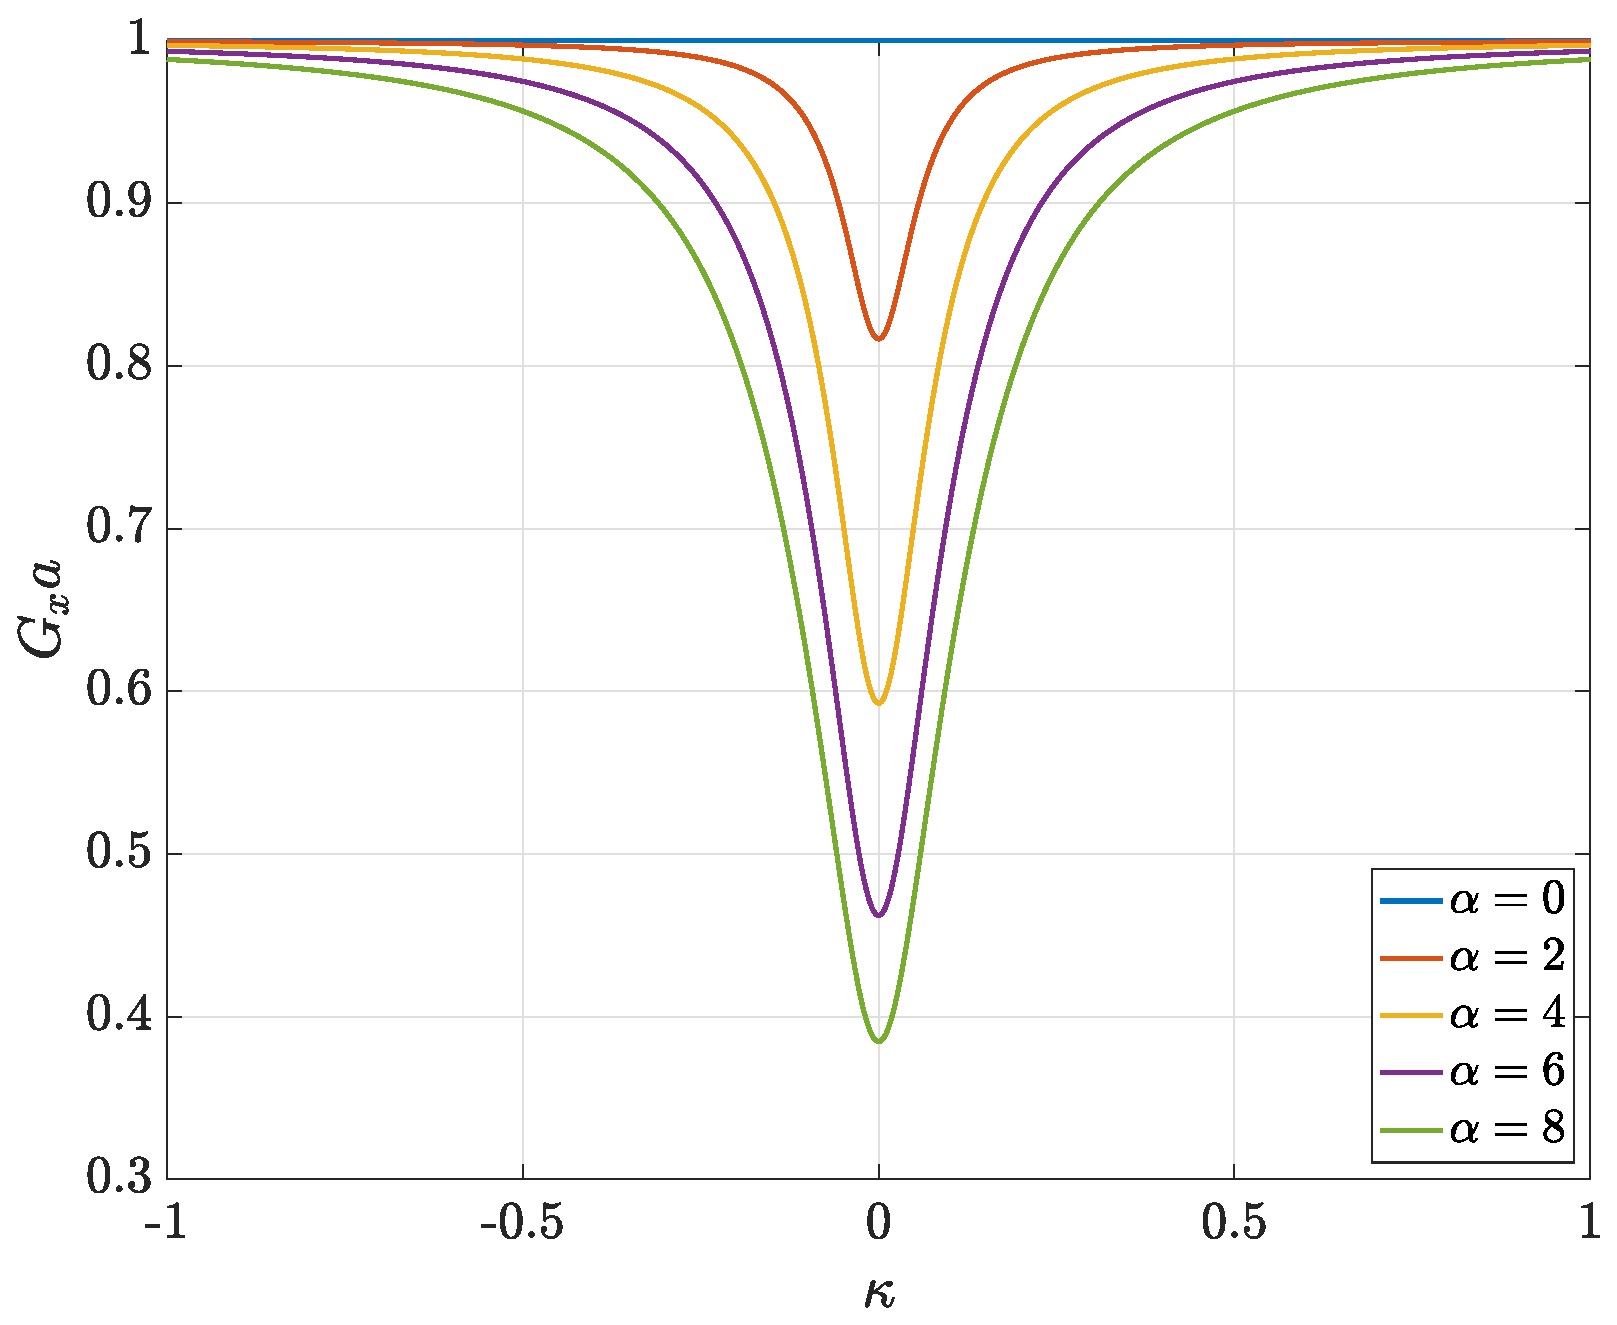
\includegraphics[scale=0.5]{ex1/e-17.eps}
        \centering
        \caption{Weighing function $\gxa$\ as a function of $\kappa$}
        \label{wf}
        \end{figure}
